\documentclass[a4paper]{standalone}
\usepackage{amsmath}
\usepackage{circuitikz}
\usetikzlibrary{fit, shapes, arrows, patterns, decorations.text, decorations.markings}

\begin{document}
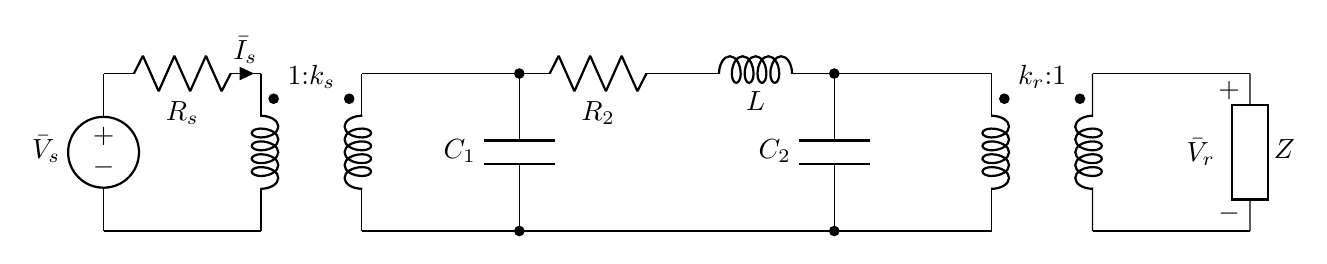
\begin{tikzpicture}[scale=1.00, transform shape, /tikz/circuitikz/bipoles/length=1.50cm, american currents, american voltages, voltage dir=RP]
  \coordinate (1) at (0,2);
  \coordinate (0) at (0,0);
  \coordinate (2) at (2,2);
  \coordinate (3) at (3.28,2);
  \coordinate (0_3) at (3.28,0);
  \coordinate (0_2) at (2,0);
  \coordinate (4) at (5.28,2);
  \coordinate (0_4) at (5.28,0);
  \coordinate (5) at (7.28,2);
  \coordinate (6) at (9.28,2);
  \coordinate (0_6) at (9.28,0);
  \coordinate (7) at (11.28,2);
  \coordinate (0_7) at (11.28,0);
  \coordinate (8) at (12.56,2);
  \coordinate (0_8) at (12.56,0);
  \coordinate (9) at (14.56,2);
  \coordinate (0_9) at (14.56,0);
  \draw (0) to [V, l^={$\bar{V}_s$}, n=V] (1);
  \draw (1) to [R, i={$\bar{I}_s$}, l_=$R_{s}$, n=R1] (2);
   \draw[] (2) to [inductor, scale=1.0] (0_2);
   \draw[] (0_3) to [inductor, scale=1.0] (3);
  \draw (2.16,1.68) node[circ] {};
  \draw (3.12,1.68) node[circ] {};
  \draw (2.64,1.96) node[minimum width=0.5] (TF) {1:$k_s$};
  \draw[-] (0) to [short, n=Wanon1] (0_2);
  \draw[-] (3) to [short, n=Wanon2] (4);
  \draw (4) to [C, l_=$C_{1}$, n=C1] (0_4);
  \draw[-] (0_3) to [short, n=Wanon3] (0_4);
  \draw (4) to [R, l_=$R_{2}$, n=R2] (5);
  \draw (5) to [L, l_=$L$, n=L] (6);
  \draw (6) to [C, l_=$C_{2}$, n=C2] (0_6);
  \draw[-] (0_4) to [short, n=Wanon4] (0_6);
  \draw[-] (6) to [short, n=Wanon5] (7);
  \draw[-] (0_6) to [short, n=Wanon6] (0_7);
   \draw[] (7) to [inductor, scale=1.0] (0_7);
   \draw[] (0_8) to [inductor, scale=1.0] (8);
  \draw (11.44,1.68) node[circ] {};
  \draw (12.4,1.68) node[circ] {};
  \draw (11.92,1.96) node[minimum width=0.5] (TF2) {$k_r$:1};
  \draw[-] (8) to [short, n=Wanon7] (9);
  \draw (9) to [generic, l=$Z$, n=Z, v=$\bar{V}_r$] (0_9);
  \draw[-] (0_8) to [short, n=Wanon8] (0_9);
  \draw (4) node[circ] {};
  \draw (0_4) node[circ] {};
  \draw (6) node[circ] {};
  \draw (0_6) node[circ] {};
\end{tikzpicture}\\



\end{document}